\documentclass[../../../main.tex]{subfiles}
\begin{document}

%%%%%%%%%%%%%%%%%%%%%%%%%%%%%%%%%%%%%%%%%
%%%%%%%%%%%%%%%%%%%%%%%%%%%%%%%%%%%%%%%%%
%%%%%%%%%%%%%%%%%%%%%%%%%%%%%%%%%%%%%%%%%
\chapter{Continuous uniform distributions}

A uniform distribution is a distribution where every possible outcome is just as likely as the others. We have seen examples of this with discrete outcomes already. 

\begin{itemize}
  \item Flipping a (fair) coin. It is just as likely to get heads as it is tails.
  \item Rolling a (fair) six-sided die. It is just as likely to roll any one of the numbers as it is any of the others.
\end{itemize}

\noindent
Those examples involve discrete outcomes. But we can have a uniform distribution for continuous outcomes too. 


%%%%%%%%%%%%%%%%%%%%%%%%%%%%%%%%%%%%%%%%%
%%%%%%%%%%%%%%%%%%%%%%%%%%%%%%%%%%%%%%%%%
\section{An example}

Suppose we measure how long it takes the drivers for a ride sharing company to give rides from one point to another. Suppose we measure 10 separate (randomly selected) rides, and we find that the times (in minutes) are these:

\begin{center}
  \begin{tabular}{|| l | l || l | l |}
    \hline
    \textbf{Ride} & \textbf{Duration} & \textbf{Ride} & \textbf{Duration} \\ \hline
    1 & 2.346 & 6 & 4.234 \\ \hline
    2 & 3.359 & 7 & 6.766 \\ \hline
    3 & 5.763 & 8 & 5.403 \\ \hline
    4 & 4.649 & 9 & 6.978 \\ \hline
    5 & 7.233 & 10 & 2.886 \\ \hline
  \end{tabular}
\end{center}


%%%%%%%%%%%%%%%%%%%%%%%%%%%%%%%%%%%%%%%%%
\subsection{The wrong way to think about it}

What is the probability of each of the above outcomes? It might be tempting to consider each of those values as a unique outcome, and count up how often each one occurs. That is, we could make a frequency table:

\begin{center}
  \begin{tabular}{|| l | l || l | l |}
    \hline
    \textbf{Outcome} & \textbf{Count} & \textbf{Outcome} & \textbf{Count}  \\ \hline
    2.346 & 1 & 5.403 & 1 \\ \hline
    2.886 & 1 & 5.763 & 1 \\ \hline
    3.359 & 1 & 6.766 & 1 \\ \hline
    4.234 & 1 & 6.978 & 1 \\ \hline
    4.649 & 1 & 7.233 & 1 \\ \hline
  \end{tabular}
\end{center}

Each one of these outcomes occurs only once. And since there are 10 observations in all, we might think that the probability of each particular outcome is one in ten, or .1.

But, this is not correct. Notice that each outcome happens only once. That tells us something. It tells us that each outcome seems just as likely as any of others. In other words, we are working with a \vocab{uniform} distribution here.

Furthermore, why should each outcome be equally likely? A hint comes from the decimal points in the values. Each outcome is a very specific measurement of time. 2.346 seconds, or 4.649 seconds, for example. 

What this tells us is that we are working with a continuous scale of time. And that means that, beyond the 10 particular time measurements we collected from our observations, there are infinitely more points of time between each of the ones that we recorded.

So counting up the outcomes in a frequency table is incorrect. A frequency table reports all the possible outcomes and how many times each one occurred. In the frequency table above, there are only 10 outcomes listed. But that's not correct. There are infinitely many other points of time that we could have observed, and we have omitted all those values from the frequency table.

So really, we are looking at a huge number of possible times. And that means that the probability of each of our observed outcomes is \emph{not} one over 10, or 0.1.


%%%%%%%%%%%%%%%%%%%%%%%%%%%%%%%%%%%%%%%%%
%%%%%%%%%%%%%%%%%%%%%%%%%%%%%%%%%%%%%%%%%
\section{Constructing the \PDFtext/}

We said that the \PDFtext/ tells us how to draw the line for a continuous distribution. In our case, the distribution is uniform (every possibility is just as likely), so the line should be a straight, horizontal line.

The \PDFtext/ should thus tell us the height of the line. For each possible outcome, the height will be the same, since each outcome is equally likely. The formula for the height is this:

\begin{equation*}
  \Probability{\RandVarVal/} = \frac{1}{\text{range of outcomes}}
\end{equation*}

\noindent
The probability of one out of six possible outcomes is one over six (or one-sixth), since there is a range of six possible outcomes. The probability of one out of 100 possible outcomes is one over a hundred (or one-hundredth), since there is a range of one hundred possible outcomes. In this case, we have a continuous range of values, so the probability will be one over the size of that range.

How do we find the size of the range of possible outcomes? We get the min and the max observed values and treat those as the top and bottom boundaries of our range. Then we say that the possible outcomes are anything that can happen in between (and including) them.

In our observations, the lowest time we recorded is 2.346, and the highest time is 7.233. How many values are there between these two numbers? We can calculate the distance between a lower point $a$ and a higher point $b$ by subtracting $a$ from $b$:

\begin{equation*}
  \text{distance} = b - a
\end{equation*}

\noindent
In this case then, the distance between the lowest and highest points is this:

\begin{equation*}
  \text{distance} = b - a = 7.233 - 2.346 = 4.887
\end{equation*}

\noindent
So, we have a span of 4.887 minutes.

If we plug that in to our \PDFtext/ formula above, we get one over 4.887:

\begin{equation*}
  P(x) = \frac{1}{4.887} = 0.205
\end{equation*} 

\noindent
See what we did there? We find the range or distance between the highest and lowest point (using $b$ - $a$), and then the probability of any one outcome is $1$ over that distance. Hence, the probability of any particular outcome in a continuous uniform distribution is this:

\begin{equation*}
  \Probability{\RandVarVal/} = \frac{1}{b - a}
\end{equation*} 


%%%%%%%%%%%%%%%%%%%%%%%%%%%%%%%%%%%%%%%%%
%%%%%%%%%%%%%%%%%%%%%%%%%%%%%%%%%%%%%%%%%
\section{Plotting it}

Let's draw a polygon plot for a continuous uniform distribution. The height is the probability, and the width is however much space is needed for the range of values. Like this:

\begin{center}
  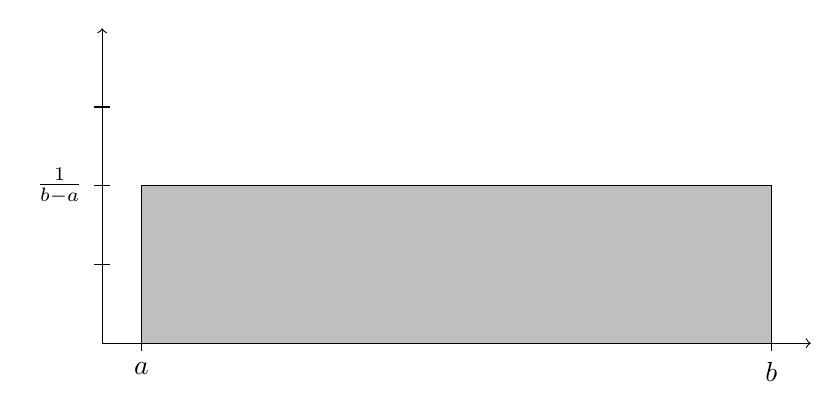
\begin{tikzpicture}

    \draw[->] (0, 0) -- (0, 4);
    \draw (-0.1, 1) -- (0.1, 1);
    \node (ytick1) at (0, 1) {};
    \draw (-0.1, 2) -- (0.1, 2);
    \node (ytick2) at (0, 2) [label=left:{$\frac{1}{b - a}$}] {};
    \draw (-0.1, 3) -- (0.1, 3);
    \node (ytick3) at (0, 3) [] {};

    \draw[->] (0, 0) -- (9, 0);
    \draw (0.5, -0.1) -- (0.5, 0.1);
    \node (xtick1) at (0.5, 0) [label=below:{$a$}] {};
    \draw (8.5, -0.1) -- (8.5, 0.1);
    \node (xtick3) at (8.5, 0) [label=below:{$b$}] {};

    \draw[fill=lightgray] (0.5, 2) -- (8.5, 2) -- (8.5, 0) -- (0.5, 0) -- (0.5, 2);

  \end{tikzpicture}
\end{center}

\noindent
In our case, the probability is 0.205, and $a$ and $b$ are 2.346 and 7.233, respectively:

\begin{center}
  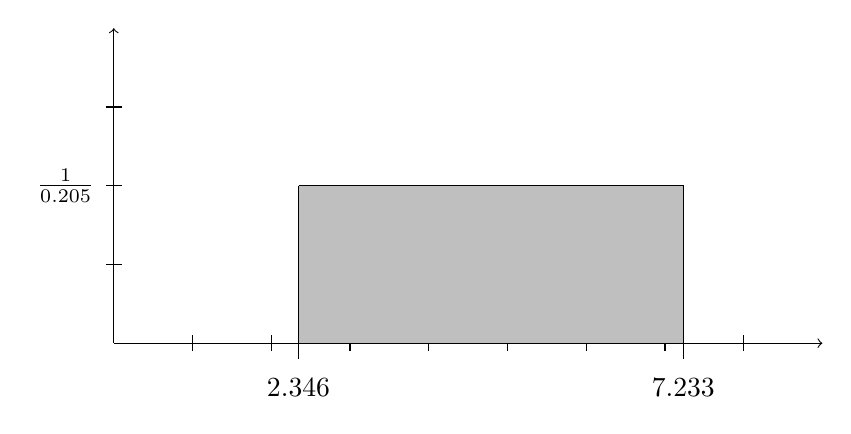
\begin{tikzpicture}

    \draw[->] (0, 0) -- (0, 4);
    \draw (-0.1, 1) -- (0.1, 1);
    \node (ytick1) at (0, 1) {};
    \draw (-0.1, 2) -- (0.1, 2);
    \node (ytick2) at (0, 2) [label=left:{$\frac{1}{0.205}$}] {};
    \draw (-0.1, 3) -- (0.1, 3);
    \node (ytick3) at (0, 3) [] {};

    \draw[->] (0, 0) -- (9, 0);
    \draw (1, -0.1) -- (1, 0.1);
    \draw (2, -0.1) -- (2, 0.1);
    \draw (3, -0.1) -- (3, 0.1);
    \draw (4, -0.1) -- (4, 0.1);
    \draw (5, -0.1) -- (5, 0.1);
    \draw (6, -0.1) -- (6, 0.1);
    \draw (7, -0.1) -- (7, 0.1);
    \draw (8, -0.1) -- (8, 0.1);
    
    \draw (2.346, -0.2) -- (2.346, 0.2);
    \node (xtick1) at (2.346, -0.2) [label=below:{$2.346$}] {};
    \draw (7.233, -0.2) -- (7.233, 0.2);
    \node (xtick3) at (7.233, -0.2) [label=below:{$7.233$}] {};

    \draw[fill=lightgray] (2.346, 2) -- (7.233, 2) -- (7.233, 0) -- (2.346, 0) -- (2.346, 2);

  \end{tikzpicture}
\end{center}


%%%%%%%%%%%%%%%%%%%%%%%%%%%%%%%%%%%%%%%%%
%%%%%%%%%%%%%%%%%%%%%%%%%%%%%%%%%%%%%%%%%
\section{The area}

We said that the area of a polygon plot represents probability exactly. We can see that here.

The probabilities of all possible outcomes should add up to 1 (100\%). So, the entire rectangle should add up to 1 as well.

How do we calculate the area of a rectangle? We multiply the width by the height (we also call the width the ``base''):

\begin{equation*}
  \text{area} = \text{base} * \text{height}
\end{equation*}

\noindent
In our case, the base is $b - a$, or $7.233 - 2.346$, which is 4.887, and the height is $\frac{1}{b - a}$, which is $\frac{1}{4.887}$, which is 0.205. So the area of the rectangle is this:

\begin{equation*}
  \text{area} = 4.887 * 0.205 = 1
\end{equation*}

\noindent
Indeed, we can see that the total area of the rectangle is 1 (plus or minus some minute decimal places, for rounding errors).


%%%%%%%%%%%%%%%%%%%%%%%%%%%%%%%%%%%%%%%%%
%%%%%%%%%%%%%%%%%%%%%%%%%%%%%%%%%%%%%%%%%
\section{Portions of the rectangle}

What is the probability that the next ride will take 5 minutes or less? How do we calculate that?

We draw a line at the 5 minute mark on the plot, and we calculate the area of everything less than that in the rectangle:

\begin{center}
  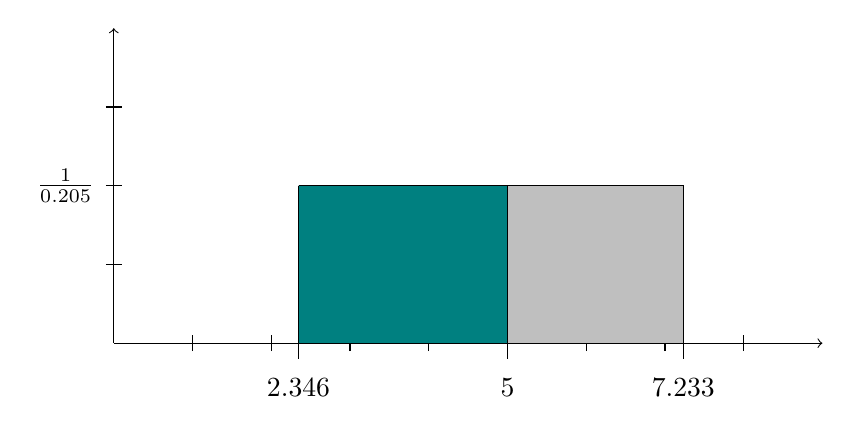
\begin{tikzpicture}

    \draw[->] (0, 0) -- (0, 4);
    \draw (-0.1, 1) -- (0.1, 1);
    \node (ytick1) at (0, 1) {};
    \draw (-0.1, 2) -- (0.1, 2);
    \node (ytick2) at (0, 2) [label=left:{$\frac{1}{0.205}$}] {};
    \draw (-0.1, 3) -- (0.1, 3);
    \node (ytick3) at (0, 3) [] {};

    \draw[->] (0, 0) -- (9, 0);
    \draw (1, -0.1) -- (1, 0.1);
    \draw (2, -0.1) -- (2, 0.1);
    \draw (3, -0.1) -- (3, 0.1);
    \draw (4, -0.1) -- (4, 0.1);
    \draw (5, -0.2) -- (5, 0.1);
    \draw (6, -0.1) -- (6, 0.1);
    \draw (7, -0.1) -- (7, 0.1);
    \draw (8, -0.1) -- (8, 0.1);
    
    \draw (2.346, -0.2) -- (2.346, 0.2);
    \node (xtick1) at (2.346, -0.2) [label=below:{$2.346$}] {};
    \draw (7.233, -0.2) -- (7.233, 0.2);
    \node (xtick2) at (7.233, -0.2) [label=below:{$7.233$}] {};

    \draw[fill=lightgray] (2.346, 2) -- (7.233, 2) -- (7.233, 0) -- (2.346, 0) -- (2.346, 2);
    \draw (5, 2) -- (5, 0);
    \node (xtick3) at (5, -0.2) [label=below:{$5$}] {};
    \draw[fill=teal] (2.346, 2) -- (5, 2) -- (5, 0) -- (2.346, 0) -- (2.346, 2);

  \end{tikzpicture}
\end{center}

To compute the area of the highlighted portion, we again use the $\text{base} * \text{height}$ formula. First, we calculate the base with $b - a$, just as before, but this time, although $a$ is still 2.346, $b$ is now $5$:

\begin{equation*}
  \text{base} = 5 - 2.346 = 2.654
\end{equation*}

The height is still the same, namely $\frac{1}{4.887}$, or $0.205$. So the area of our desired chunk of the rectangle is this:

\begin{equation*}
  \text{area} = 2.654 * 0.205 = 0.544
\end{equation*}

So the probability of the next bus ride taking 5 minutes or less is .544, or 54.4\%. If you think about it, that makes sense. The lowest time for a bus ride is a little over 2 minutes, and the longest time for a bus ride is a little over 7 minutes, so we would expect the middle point to fall somewhere in the middle, a little over 4.5. (To be exact, the mid point is 4.7895.) So, 5 minutes is a little past the middle point in the range, which makes it clear why the highlighted portion of the plot above takes up about 54\% of the whole rectangle. 

We could follow the same procedure to find the probability of the next bus ride taking six or more minutes:

\begin{center}
  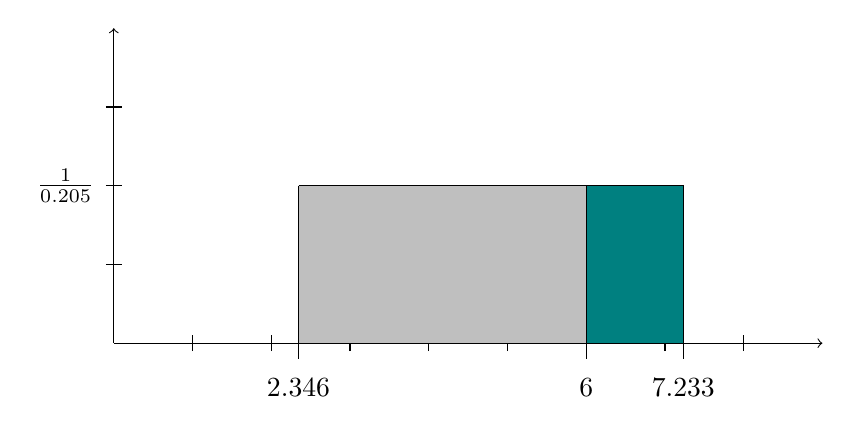
\begin{tikzpicture}

    \draw[->] (0, 0) -- (0, 4);
    \draw (-0.1, 1) -- (0.1, 1);
    \node (ytick1) at (0, 1) {};
    \draw (-0.1, 2) -- (0.1, 2);
    \node (ytick2) at (0, 2) [label=left:{$\frac{1}{0.205}$}] {};
    \draw (-0.1, 3) -- (0.1, 3);
    \node (ytick3) at (0, 3) [] {};

    \draw[->] (0, 0) -- (9, 0);
    \draw (1, -0.1) -- (1, 0.1);
    \draw (2, -0.1) -- (2, 0.1);
    \draw (3, -0.1) -- (3, 0.1);
    \draw (4, -0.1) -- (4, 0.1);
    \draw (5, -0.1) -- (5, 0.1);
    \draw (6, -0.2) -- (6, 0.1);
    \draw (7, -0.1) -- (7, 0.1);
    \draw (8, -0.1) -- (8, 0.1);
    
    \draw (2.346, -0.2) -- (2.346, 0.2);
    \node (xtick1) at (2.346, -0.2) [label=below:{$2.346$}] {};
    \draw (7.233, -0.2) -- (7.233, 0.2);
    \node (xtick2) at (7.233, -0.2) [label=below:{$7.233$}] {};

    \draw[fill=lightgray] (2.346, 2) -- (7.233, 2) -- (7.233, 0) -- (2.346, 0) -- (2.346, 2);
    \draw (6, 2) -- (6, 0);
    \node (xtick3) at (6, -0.2) [label=below:{$6$}] {};
    \draw[fill=teal] (6, 2) -- (7.233, 2) -- (7.233, 0) -- (6, 0) -- (6, 2);

  \end{tikzpicture}
\end{center}

The base of the section we care about is now $7.233 - 6$:

\begin{equation*}
  \text{base} = 7.233 - 6 = 1.233
\end{equation*}

And the height is still the same, so the area is $\text{base} * \text{height}$:

\begin{equation*}
  \text{area} = 1.233 * 0.205 = 0.253
\end{equation*}

Hence, the probability of the next bus ride taking 6 or more minutes is 0.253. Again, this looks about right. In the plot, about 25\% of the whole rectangle is highlighted.

\end{document}
